\documentclass[t]{beamer}
\usepackage{listings}
\usepackage{minted}

\usetheme{default}
\usebackgroundtemplate{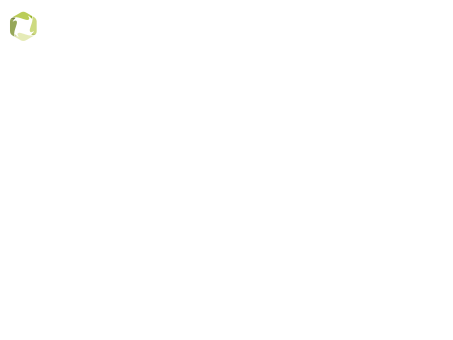
\includegraphics[width=\paperwidth]
                                       {../cpeb_bkground_topleftlogo.pdf}}

\setbeamertemplate{frametitle}{
  \centering\vspace{1mm}\insertframetitle\par\vspace{3mm}
}

\usepackage[style=nature,
            hyperref,
            backend=biber,
            isbn=false,
            doi=false,
            url=false,
            date=year,
            maxbibnames=3
           ]{biblatex}

\bibliography{kwip-tic.bib}

\title{\texttt{kWIP}: The k-mer Weighted Inner Product}
\author{Kevin Murray}
\institute{PhD Candidate, Borevitz Lab, CPEB, ANU}
\date{21 August 2015}

\usefonttheme{serif}

\begin{document}

{
\usebackgroundtemplate{
\includegraphics[width=\paperwidth]{../cpeb_bkground_centered.pdf}}
\begin{frame}
  \titlepage
  \vfill
\end{frame}
}

\begin{frame}{Overview}
  \begin{itemize}
    \item Motivation
    \item Technological overview
    \item Early results and plans
  \end{itemize}
\end{frame}

\begin{frame}{Large-scale population genomics}
  \begin{itemize}
    \item Moving from 100s to 1,000s or 10,000s of samples \textit{per PhD!}
      \pause
    \item Efficient algorithms to analyse large-scale genomic data
    \begin{itemize}
      \item Reference \& alignment free: \textit{less bias, de novo}
      \item Platform/protocol agnostic: \textit{future proof}
      \item Computationally efficient: \textit{not the bottleneck}
      \item Cross scale: \textit{one tool to rule them all}
    \end{itemize}
  \end{itemize}
  \begin{center}
    \includegraphics[width=\textwidth]{img/cross-scale.png}
  \end{center}
  \tiny{after \textcite{peterson_double_2012}}
\end{frame}


\begin{frame}{Why Estimate Similarity?}
  \begin{itemize}
    \item Rough approximation of sample relatedness required
      \begin{itemize}
        \item For natural collections
        \item For association mapping
        \item As a technical control
      \end{itemize}
  \end{itemize}
  \pause
  \begin{center}
    \includegraphics<2>[width=\textwidth]{img/restruct-1}
    \includegraphics<3>[width=\textwidth]{img/restruct-2}
    \includegraphics<4>[width=\textwidth]{img/restruct-3}
    \includegraphics<5>[width=\textwidth]{img/restruct-4}
    \begin{itemize}
      \item[]<2-5> \tiny{after \textcite{brachi_genome-wide_2011}}
    \end{itemize}
    \includegraphics<6>[width=\textwidth]{img/jared-tree.pdf}
    \includegraphics<7>[width=0.6\textwidth]{img/at80-tree.png}
  \end{center}
\end{frame}


\begin{frame}{Presenting \texttt{kWIP}}
  \begin{itemize}
    \item $k$-mer based \textit{de novo} genetic clustering
    \item Weighted Inner Product between hashes to determine similarity
    \item Produces a distance matrix from raw NGS reads
  \end{itemize}
  \begin{center}
    \includegraphics[width=\textwidth]{img/kwip-overview.png}
  \end{center}
\end{frame}

\begin{frame}{Technological Overview}
  \begin{itemize}
    \item $k$-mer counting (bag-of-words)
    \begin{itemize}
      \item Decompose sequences to overlapping words of $k$
    \end{itemize}
    \pause
    \item Hashing and Probabilistic Data Structures
      \begin{itemize}
        \item Efficient storage \& compute of ``bag of words''
      \end{itemize}
    \pause
    \item Population and Frequency Hashes
    \pause
    \item (Weighted) Inner Products
      \begin{itemize}
        \item Similarity metric weighted by Shannon entropy
      \end{itemize}
  \end{itemize}
\end{frame}


\begin{frame}{$k$-mer based clustering}
  \begin{itemize}
    \item Alignment-free sequence clustering is a whole field
    \item $D2$ and friends
    \item Most require assembled gene/genome sequence
    \item Many use inner product as similarity measure
  \end{itemize}
  \begin{center}
    \includegraphics[width=0.6\textwidth]{img/foret-et-al-d2.png}
  \end{center}
\end{frame}

\begin{frame}{\texttt{kWIP}}
  \begin{itemize}
    \item The $k$-mer Weighted Inner Product
      \begin{itemize}
        \item Extends alignment-free seq comparison to raw NGS data
      \end{itemize}
    \pause
    \item Algorithm:
      \begin{itemize}
        \item For each run: count all $k$-mers into a hash
        \pause
        \item For each analysis set, i.e ``population'':
          \begin{itemize}
            \item Calculate the entropy of population frequency ($H$)
            \item For each pair of runs $A$ and $B$, calculate \\
              $\sum\limits^{n}_{i=0} A_i \cdot B_i \cdot H_i$
          \end{itemize}
      \end{itemize}
  \end{itemize}
  \begin{center}
    \includegraphics[width=0.4\textwidth]{img/hash-wip.png}
  \end{center}
\end{frame}


\begin{frame}{\texttt{kWIP}}
  \begin{itemize}
    \item The software:
      \begin{itemize}
        \item \texttt{C++}, $>$2000 lines of code
        \item Uses \texttt{khmer} for $k$-mer counting \& hashing
        \item Parallelised, fast
        \item GNU GPL licensed, source code on GitHub
      \end{itemize}
      \begin{center}
        \includegraphics[width=0.5\textwidth]{img/kwip-doc-screenshot.png}
      \end{center}
  \end{itemize}
\end{frame}

\begin{frame}{\texttt{kWIP} Experiments}
  \begin{itemize}
    \item 3000 rice genomes:
      \begin{itemize}
        \item 3000 rice lines from known families
        \item Analysing in sets of $\approx 100$, from all major groups
        \item Recover known grouping w/ \texttt{kWIP}, not w/ unweighted IP
        \item Sensitive to read depth
      \end{itemize}
    \item Simulation
      \begin{itemize}
        \item Fake population genome sequencing studies
      \end{itemize}
  \end{itemize}
\end{frame}

\begin{frame}{96 Rice Runs}
  \begin{itemize}
    \item Set of 96 rice runs from 16 samples (6 tech reps ea)
    \item About half/half from 2 major groups (Indica, Japonica)
    \item Expectations:
      \begin{itemize}
        \item All runs cluster into groups of 6 reps (16 samples)
        \item Big split between two groups: (7 and 9 respectively here)
      \end{itemize}
    \item We see this with \texttt{kWIP}, not with Unweighted IP
    \item Took 10 hours on 16-core Raijin node, 60-80GB RAM
  \end{itemize}
\end{frame}

\begin{frame}
  \begin{center}
    \includegraphics<1>[width=\textwidth]{img/distmat-both.png}
    \includegraphics<2>[width=\textwidth]{img/dendro-both.png}
  \end{center}
\end{frame}

\begin{frame}
  \begin{center}
    \includegraphics<1>[width=0.6\textwidth]{img/dendro-wip.png}
    \includegraphics<2>[width=0.6\textwidth]{img/dendro-ip.png}
  \end{center}
\end{frame}

\begin{frame}{Simulation}
  \begin{itemize}
    \item Aims to re-create a bifurcating tree
    \item \texttt{kWIP} does so
    \item Neighbour joining trees have Robinson-Foulds distance of 0
  \end{itemize}
  \begin{center}
    \includegraphics[width=0.8\textwidth]{img/kwip-dendro.png}
  \end{center}
\end{frame}

\begin{frame}
  \begin{center}
    \includegraphics<1>[width=0.8\textwidth]{img/true-mat.png}
    \includegraphics<2>[width=0.8\textwidth]{img/kwip-mat.png}
    \includegraphics<3>[width=0.8\textwidth]{img/ip-mat.png}
  \end{center}
\end{frame}

\begin{frame}{Conclusions}
  \begin{itemize}
    \item \texttt{kWIP} is implemented, Beta software
    \item We show the utility of \texttt{kWIP}
    \item Further simulations and experiments required
    \item Publication in preparation
  \end{itemize}
\end{frame}

\begin{frame}{Thanks}
  \begin{itemize}
    \item Supervisors: Justin, Sylvain, Gavin and Barry
    \item My collaborators: Christfried  Webers, Cheng Soon Ong, Norman Warthmann
    \item \texttt{khmer} folks: C. Titus Brown, Michael Crusoe, Camille Scott
          (DIB-lab) @ UC Davis
    \item Yourselves
  \end{itemize}
\end{frame}

\begin{frame}[shrink=20]{References}
  \printbibliography
  \vfill
  .
\end{frame}

\end{document}
